\documentclass{article}
\usepackage{microtype,graphicx,booktabs,hyperref,amsmath,amssymb}
\newcommand{\theHalgorithm}{\arabic{algorithm}}
\usepackage[preprint]{icml2026}
\icmltitlerunning{Audited Event-Time Control and Experience Admission}
\makeatletter\gdef\icmlcorrespondingauthor@text{Paper B component report}\makeatother
\hypersetup{pdftitle={Audited Event-Time Control and Experience Admission},pdfauthor={Paper B component study},pdfsubject={Mechanical simulation component note in ICML preprint format}}
\begin{document}
\twocolumn[
\icmltitle{Audited Event-Time Control and Experience Admission:\\
A Paired Mechanical Component Study}
\begin{icmlauthorlist}\icmlauthor{Paper B component study}{report}\end{icmlauthorlist}
\icmlaffiliation{report}{Simulation and evidence-interface evaluation}
\vskip .3in]
\printAffiliationsAndNotice{}

\begin{abstract}
Physical deadlines concern effects, not command receipts. We compare
four controller lifecycles under identical public models and budgets
on eight development-seen mechanical configurations.
All 32 independently audited episodes satisfy the joint contract; strong batch ties feedback and replanning on success.
Independent RAW separates onset from confirmation. Metadata validation
admits no training rows. This simulated component establishes no VLA,
chemical or agentic benefit.
\end{abstract}

\begin{figure*}[t]
\centering
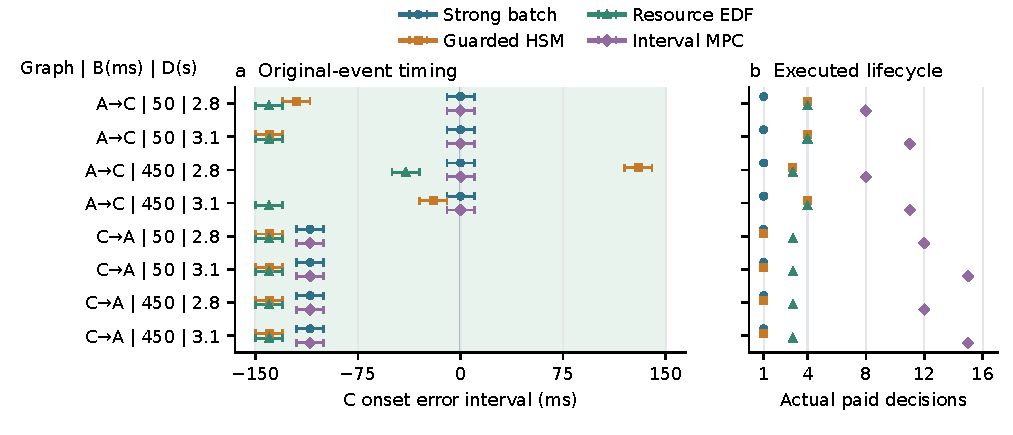
\includegraphics[width=\textwidth]{../inputs/paired32_print.pdf}
\caption{All 32 audited development episodes. Left: C onset-error intervals relative to the original B event, with the allowed $\pm150$ ms window shaded. Right: actual charged decision counts. Intervals, not midpoints, determine certification. Different workloads do not establish an agentic or statistical advantage.}
\label{fig:paired}
\end{figure*}

\section{Question and scope}
Physical-time policies \cite{chronos,timecontrol} and chemistry-twin
verifiers \cite{matterix} already exist. We compare feedback and
replanning against a strong same-information schedule, separating
physical success from learning-data eligibility.

\section{Original-event contracts}
For events $a,b$ in the same epoch, let occurrence brackets be
$I_a=[\ell_a,u_a]$, $I_b=[\ell_b,u_b]$. The conservative relative interval is
\[
 J_{b\mid a}=[\ell_b-u_a,\;u_b-\ell_a].
\]
A required window $W$ is TRUE if $J\subseteq W$, FALSE if
$J\cap W=\varnothing$, and UNKNOWN otherwise. Missing events are UNKNOWN.
The conjunction retains FALSE/UNKNOWN, refusals, exhaustion and missing
attempts in the planned denominator. A graph edge requires its minimum
gap under the same brackets; success also requires its physical predicates.

The fixture contains three contact-free MuJoCo rotors. B's first actual
$q=2$ crossing is an immutable original reference. A must stop within
$[1.8,D]$ seconds of B; C within $D\pm.15$ seconds, with a 40 ms graph gap.
B's required motion and drive profile are checked over its original
six-second interval. The RAW endpoint is the first stop with prior
movement and 21 samples at speed $\le.1$ spanning 200 ms on the 10 ms
grid. Occurrence differs from confirmation; sampled predicates do not
prove continuity between samples.

\section{Public control and paid decisions}
Actors receive lagged position, velocity, torque, capture/arrival times,
reservations and ACKs. Same-tick capture is pre-ACK; effect evidence
requires capture $\ge$ACK+10 ms. ACK is not stopping. Every actor may
conditionally refine the \emph{same} B event with the unfitted public
model. Coarse 50 ms observation is not an information lower bound;
compatibility does not certify physical support.

A capacity-one bus services A/C and B's reservation. The first A ACK
leaves A powered; public hypotheses are none/first-drop. Accepted
requests cannot be cancelled/refunded. Caps are two requests per rotor,
four total, and 1,000 candidates per decision/10,000 per epoch including
resource rejections. Each decision costs 20 ms, two native ticks;
old commitments and physics continue. Python compute otherwise pauses
physics: this charge is not LLM wall time.

\paragraph{Four distinct lifecycles.}
Strong batch commits a complete joint schedule with blind redundancy.
Guarded HSM uses a safe feedback retry slot or the same blind fallback.
EDF replans unissued requests with inherited deadlines. Interval MPC
commits one prefix and recedes on public changes or a 100 ms cadence.
The ledger charges at emission; paid replacements with stale request or
calendar history are discarded. Failed bounded search does not prove
infeasibility.

\section{Paired evidence and attribution}
Graph order, B service 50/450 ms and $D=2.8/3.1$ seconds yield eight
fixed configurations. D changes A's upper bound and C's window together.
One episode per method/configuration gives 32 episodes, eight per
method, with unique identities and the same initial state. All
configurations were previously seen; no random-seed, IID, heldout or
OOD claim follows.

\begin{table}[h]
\centering
\caption{Actual audited episodes: eight per method. T/F/U is the joint physical contract. Charge is virtual decision time.}
\label{tab:actual}
\small
\begin{tabular}{@{}lcccc@{}}
\toprule
Method & T/F/U & Dec. & Proposals & Charge (ms) \\
\midrule
Strong batch & 8/0/0 & 1 & 282--370 & 20 \\
Guarded HSM & 8/0/0 & 1--4 & 286--901 & 20--80 \\
Resource EDF & 8/0/0 & 3--4 & 284--1197 & 60--80 \\
Interval MPC & 8/0/0 & 8--15 & 1548--3131 & 160--300 \\
\bottomrule
\end{tabular}
\end{table}
All methods are 8/8 joint TRUE (Table~\ref{tab:actual}), with zero FALSE/UNKNOWN and A2/C1 requests throughout. Strong batch already explains all eight configurations; no feedback, replanning or learning benefit is demonstrated. Workloads are descriptive under shared caps. Maximum actual A/C queue waits are 0/0/20/10 ms for batch/HSM/EDF/MPC; B reservation wait is separate.

The 64 scalar software checks (8 configurations$\times$4 methods$\times$2
fault hypotheses) all pass, including batch; they are not native
episodes. The separate native prerequisite is TRUE, with one primary
and one diagnostic re-integration, 1,201 samples/1,200 steps each.
It is not a paired32 outcome.
The 32 controlled episodes contain 38,432 RAW samples/38,400 steps. Separately, 32 diagnostic command re-integrations add 38,432 samples/38,400 steps with zero state/time error. Replays are not new primary trials.

\section{Evidence admission is not learning}
The replay interface preserves four legacy calibration, sixteen test
and eight development records: 28 metadata records, not new robot tests.
Its 852 image-action candidates have 832 UNKNOWN policy-image delivery
times and 20 REJECTED tail frames with no future submission. Applied
control or post-hoc effect is not a future submission label. Thirty-four
CPU schema/cross-field checks and clean public metadata replay pass;
student tensors and DP/offline-RL/OPD training rows remain zero. This
metadata gate postdates the legacy outcomes.

The actors are rules, not neural teachers; aggregation without student
rollouts is not on-policy distillation. Learning requires causal
observations, learner-state labels, matched budgets and unseen tests.
Loaded stirring, flow, heating and chemical endpoints need separate
validation. This study uses no GPU, LLM calls or weight updates.

\begin{thebibliography}{9}
\bibitem[Darvish et~al.(2026)]{matterix}
Darvish, K. et~al. MATTERIX: toward a digital twin for robotics-assisted
chemistry laboratory automation. \emph{Nature Computational Science},
6:67--82, 2026.
\href{https://doi.org/10.1038/s43588-025-00924-4}{doi:10.1038/s43588-025-00924-4}.
\bibitem[Jia and Chen(2026)]{timecontrol}
Jia, Y. and Chen, B. Time as a Control Dimension in Robot Learning.
\href{https://arxiv.org/abs/2511.07654}{arXiv:2511.07654}, version 2, 2026.
\bibitem[Wang et~al.(2026)]{chronos}
Wang, C., Clark, J., and Song, S.
Chronos Policy: Learning Robot Policies on Physical Time.
\href{https://arxiv.org/abs/2610.13929}{arXiv:2610.13929}, 2026.
\end{thebibliography}
\end{document}
